
%version 2: \usepackage{hyperref}


%%%%%%%%%%%%%%%%%%%%%%%%%%%%%%%%%%%%%%%%%%%%%%%%%%%%%%%%%%%%%%%%%%%%%%%%
%Para las ecuaciones siempre es Ec.(n).
%Para las figuras siempre es Fig.n, incluso en el caption de la figura. Tambien las Tablas
%Para las referencias es [n]
%%%%%%%%%%%%%%%%%%%%%%%%%%%%%%%%%%%%%%%%%%%%%%%%%%%%%%%%%%%%%%%%%%%%%%%%

\documentclass[
reprint,
%notitlepage,
%superscriptaddress,
%groupedaddress,
%unsortedaddress,
%runinaddress,
%frontmatterverbose, 
%preprint,
%showpacs,preprintnumbers,
%nofootinbib,
%nobibnotes,
%bibnotes,
%11 pt,
amsmath,
amssymb,
%aps,
%pra,
prb,
%rmp,
%tightenlines %esto hizo el milagro de sacar los espacios en blancos estocásticos (?)
%prstab,
%prstper,
%floatfix,\textbf{}
]{revtex4-1} %Instalar primero para usarlo. Paquete malo.

%\documentclass[onecolumn, aps, amsmath,amssymb ]{article}
\usepackage{lipsum}  
\usepackage{graphicx}% Include figure files
\usepackage{subfig}
\usepackage{braket}
\usepackage{comment} %comment large chunks of text
\usepackage{dcolumn}% Align table columns on decimal point
\usepackage{bm}% bold math
%\usepackage{hyperref}% add hypertext capabilities
\usepackage[mathlines]{lineno}% Enable numbering of text and display math
%\linenumbers\relax % Commence numbering lines
\usepackage{mathtools} %% Para el supraíndice

\usepackage[nice]{nicefrac}

%%%%%%%El Señor Español%%%%%%%%%%%%%%%%%%%%%%%%%%%
\usepackage[utf8]{inputenc} %acento
\usepackage[
spanish, %El lenguaje.
es-tabla, %La tabla y no cuadro.
activeacute, %El acento.
es-nodecimaldot %Punto y no coma con separador de números
]{babel}
\usepackage{microtype} %para hacerlo más bonito :33 como vos (?) 
%%%%%%%%%%%%%%%%%%%%%%%%%%%%%%%%%%%%%%%%%%%%%%%%%%%
%%%%%%%%% Para que las imágenes se queden dónde las quiero (?
\usepackage{float}
%%%%%%%%%%
\usepackage{enumitem}
\usepackage{hyperref} % Para usar \url

%%%%%%%%Cambia a Fig de Figure%%%%%%%%%%
\makeatletter
\renewcommand{\fnum@figure}{Fig. \thefigure} 
\makeatother
%%%%%%%%%%%%%%%%%%%%%%%%%%%%%%%%%%%%%%%%
\raggedbottom



   %\usepackage[caption=false]{subcaption}

\begin{document}
%%%%%%%%%%%%%%%%%%%%%%%%%%%%%%%%%%Título%%%%%%%%%%%%%%%%%%%%%%%%%%%%%%%%%%%%%%
%%%%%%%%%%%%%%%%%%%%%%%%%%%%%%%%%%%%%%%%%%%%%%%%%%%%%%%%%%%%%%%%%%%%%%%%%%%%%%

\title{Práctica 1: Redes Neuronales y Aprendizaje Profundo para Visión Artificial}
\author{Evelyn~G.~Coronel}

\affiliation{
Aprendizaje Profundo y Redes Neuronales Artificiales\\ Instituto Balseiro\\}

\date[]{\lowercase{\today}} %%lw para lw, [] sin date


\maketitle
%\onecolumngrid


\section*{Ejercicio 1}

En este ejercicio se implementó una regresión lineal de la  para un cantidad N de puntos en d dimensiones.  Para realizar este ejercicio se generan los valores de $x_i$ y $a_{m,exacto}$ de forma aleatoria entre $[-4,4]$. se calcula el valor
\begin{equation}
  y_i= \sum_{i=1}^d a_{i,esperado}x_i+ a_0 + \epsilon[-1,1]  
\end{equation}
donde se agrega un ruido uniforme que varía entre $[-1,1]$

Una vez obtenido el conjunto de datos $X$, se calculan  los parámetros esperados de la regresión lineal mediante la Ec.\,\ref{eq:ejer1}

\begin{equation}
     \vec a_{esperado} = (X^TX)^{-1}X^T \vec y,
     \label{eq:ejer1}
 \end{equation} 
donde $\vec a$ representa a $\{a_i, a_0 \}$, $X$ es la representación matricial de datos e $\vec y$ son los valores $y_i$.

En las Figs.  \ref{fig:ejer1_a_ejemplos} y \ref{fig:ejer1_y_ejemplos}  se muestran los errores cuadráticos medios  (MSE) en función de la cantidad de ejemplos dados para calcular los parámetros del problema (\ref{fig:ejer1_a_ejemplos}), así también de la salida (\ref{fig:ejer1_y_ejemplos}). 

Se observa  para una dimensión fija, el MSE disminuye a medida que se aumenta la cantidad de ejemplos para calcular los parámetros. En las mismas figuras se observa un subfigura donde se muestra como varía el valor de MSE fijando la cantidad de ejemplos, donde el error también aumenta con la dimensión.

Esto indica que a medida que voy a aumentando la dimensión del problema voy a necesitar más ejemplos para obtener un error menor. Como se muestra en las subfiguras,  la diferencia entre los errores  aumenta con la dimensión, comparando dos cantidades de ejemplos.

Más aún, si consideramos un valor de MSE fijo, por ejemplo en la Fig.\ref{fig:ejer1_y_ejemplos} con $MSE\approx 0.5$, con $d=80$ se necesitaron $\sim 180$ ejemplos para llegar a ese error,para  $d=120$ se necesitaron $\sim 270$ y para $d=160$ se necesitaron $\sim 380$  ejemplos. Por lo que se puede decir que:

\begin{equation}
    \frac{\Delta d}{\Delta N} \approx   0.5 \times N
\end{equation}
 necesita más ejemplos que la diferencia entre dimensiones



    \begin{figure}[H]
        \centering
        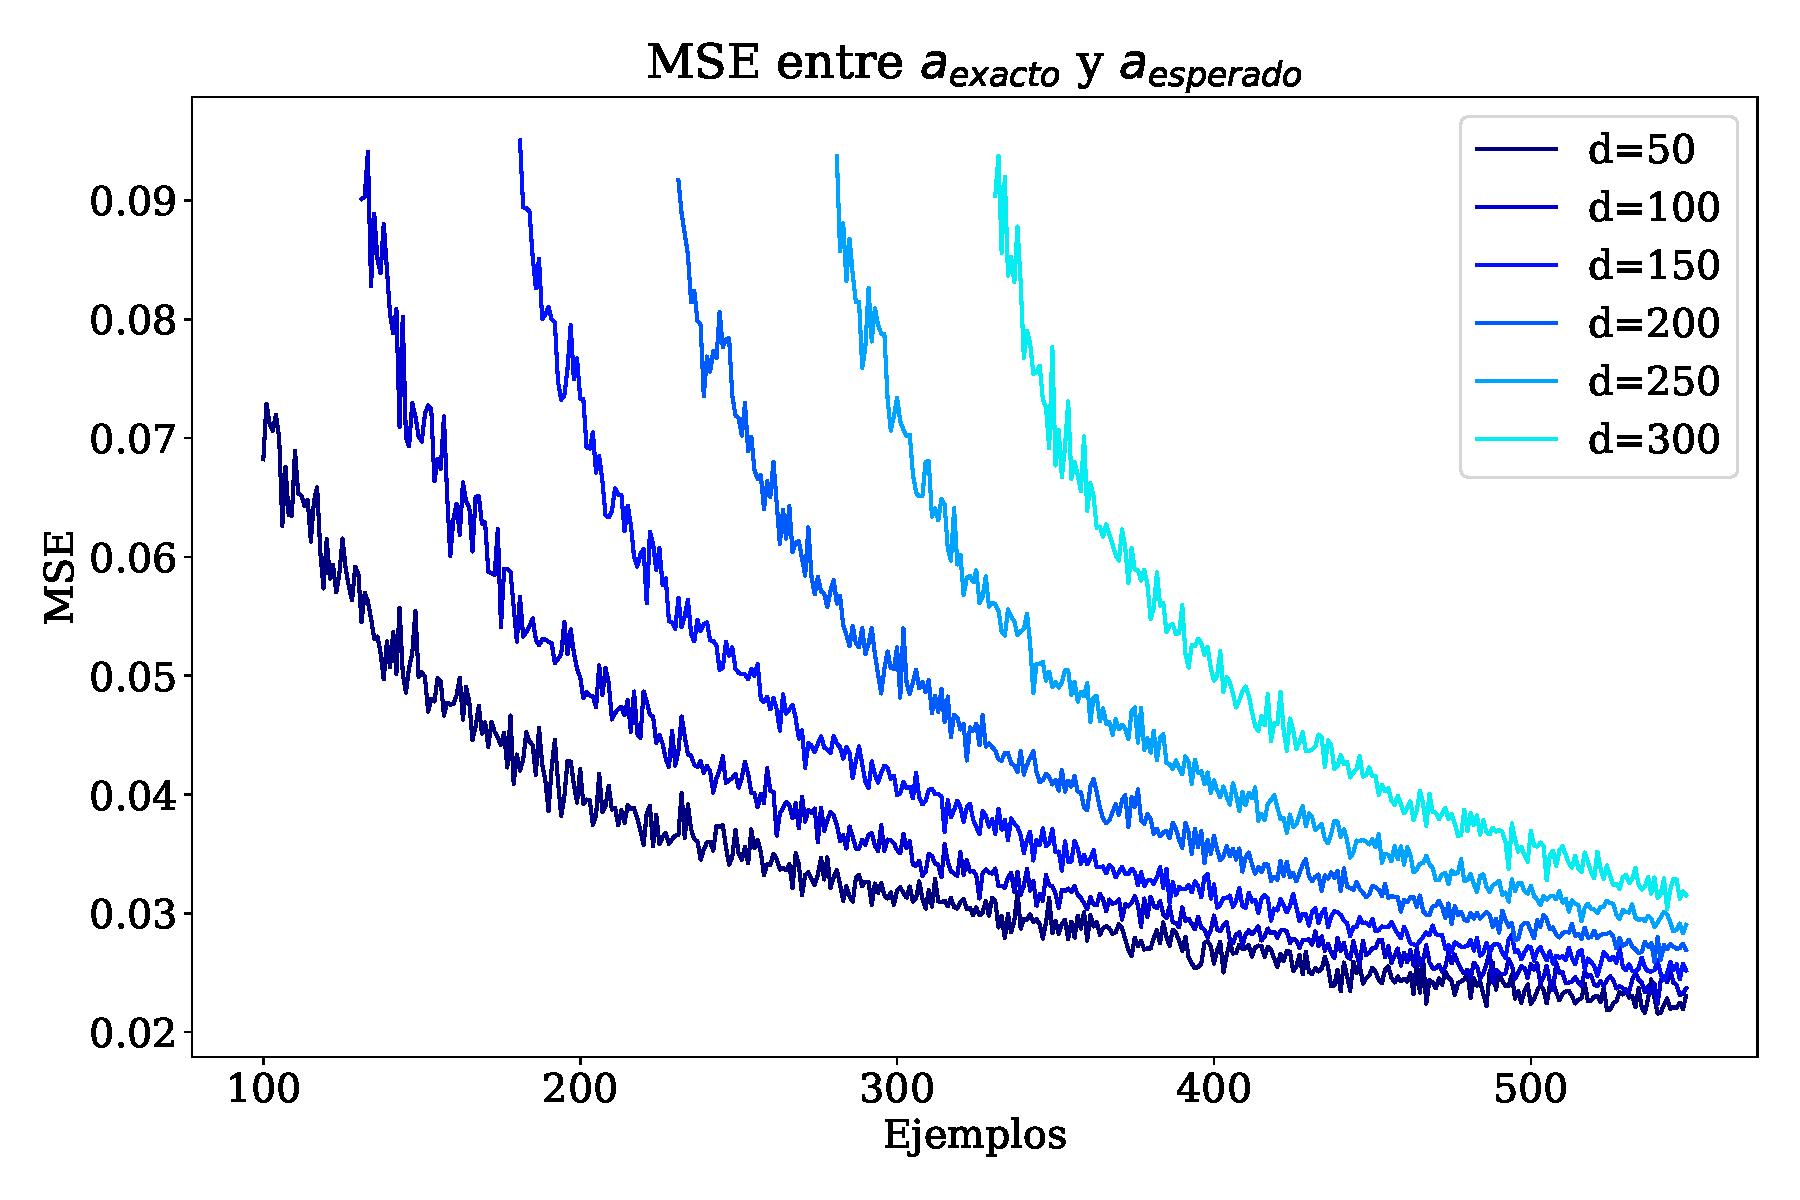
\includegraphics[width=0.49\textwidth]{plots/ejer_1_mse_a_ejemplos.pdf}
        \caption{ejemplos}
        \label{fig:ejer1_a_ejemplos}
    \end{figure}


    \begin{figure}[H]
        \centering
        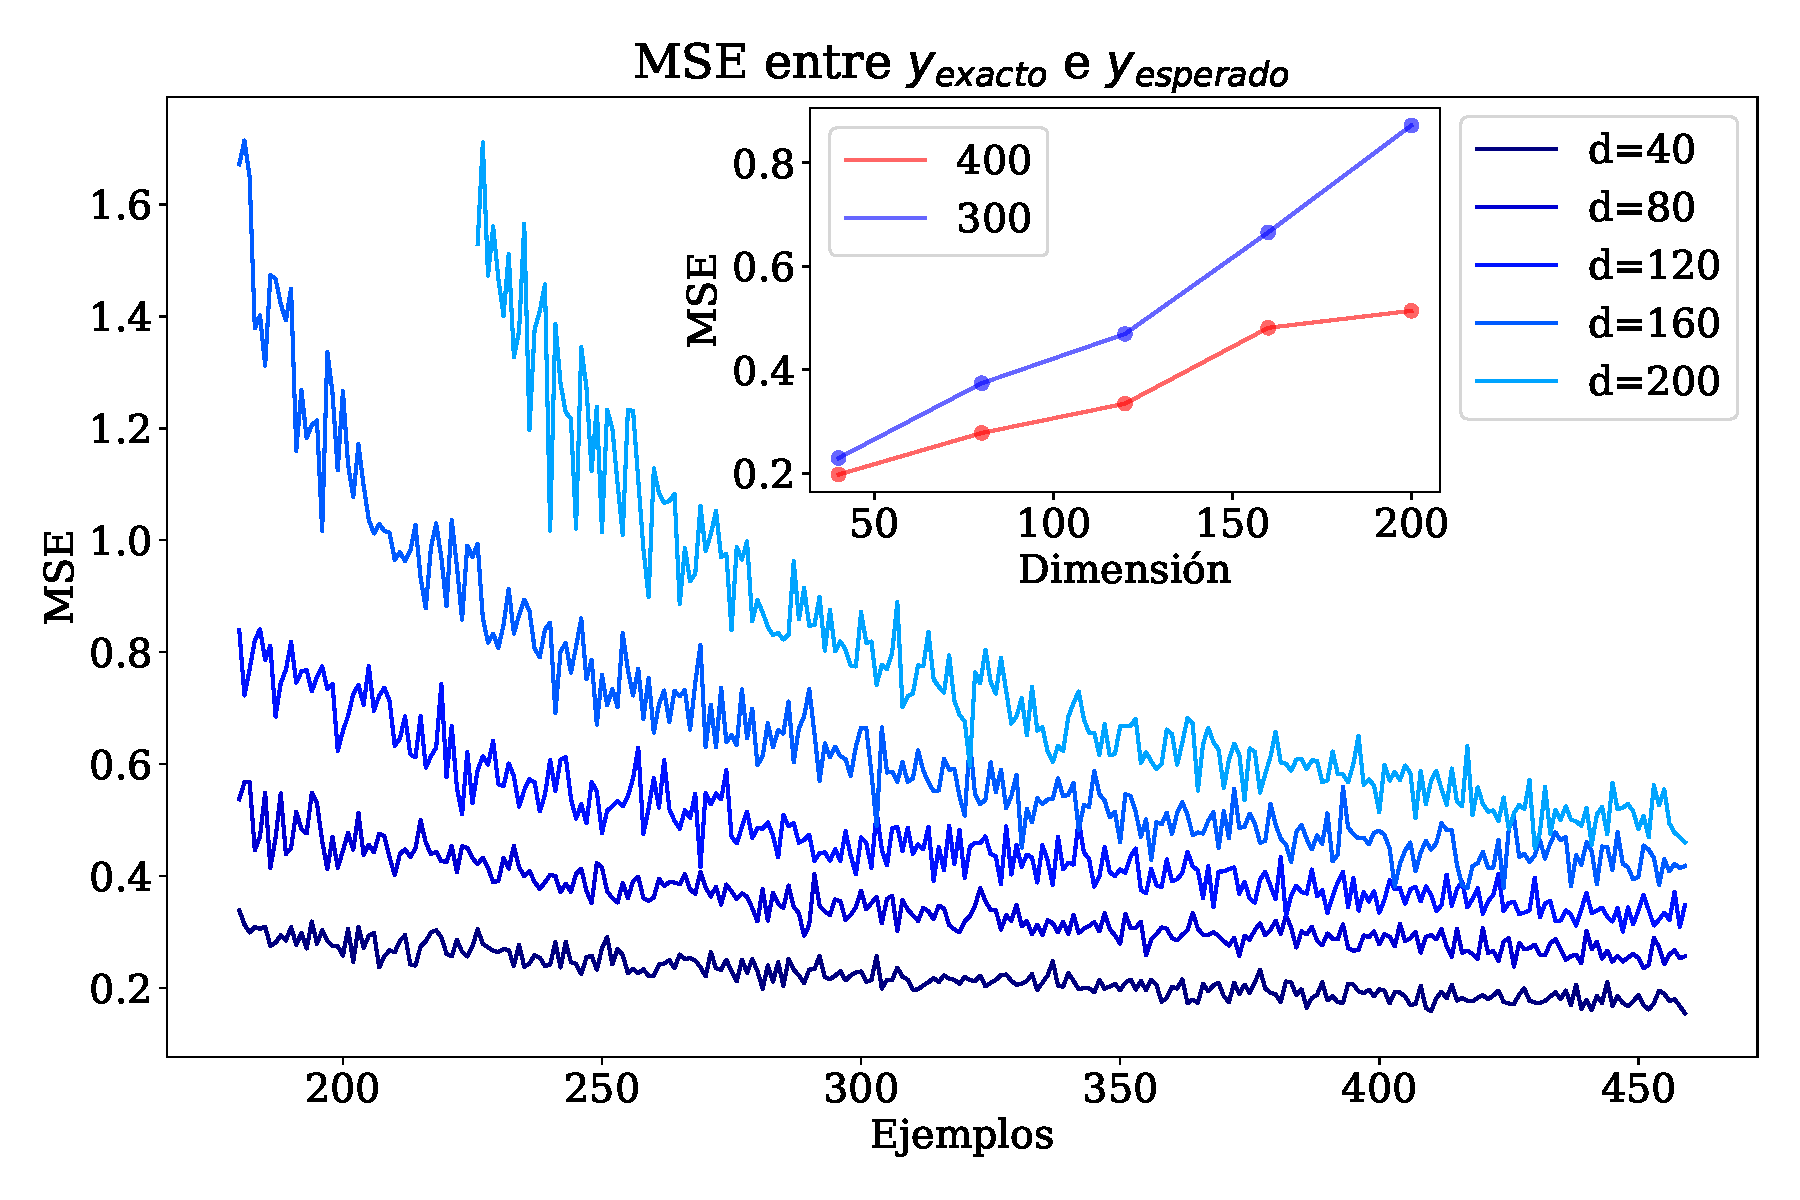
\includegraphics[width=0.5\textwidth]{plots/ejer_1_mse_y_ejemplos.pdf}
        \caption{ejemplos}
        \label{fig:ejer1_y_ejemplos}
    \end{figure}

    \section*{Ejercicio 2}

    Las medias y las desviaciones estándar de cada clase fueron inicializadas de manera aleatoria

    Los gráficos se hicieron con d=7 y p=4


    Esto es un ejemplo que converge
    \begin{figure}[H]
        \centering
        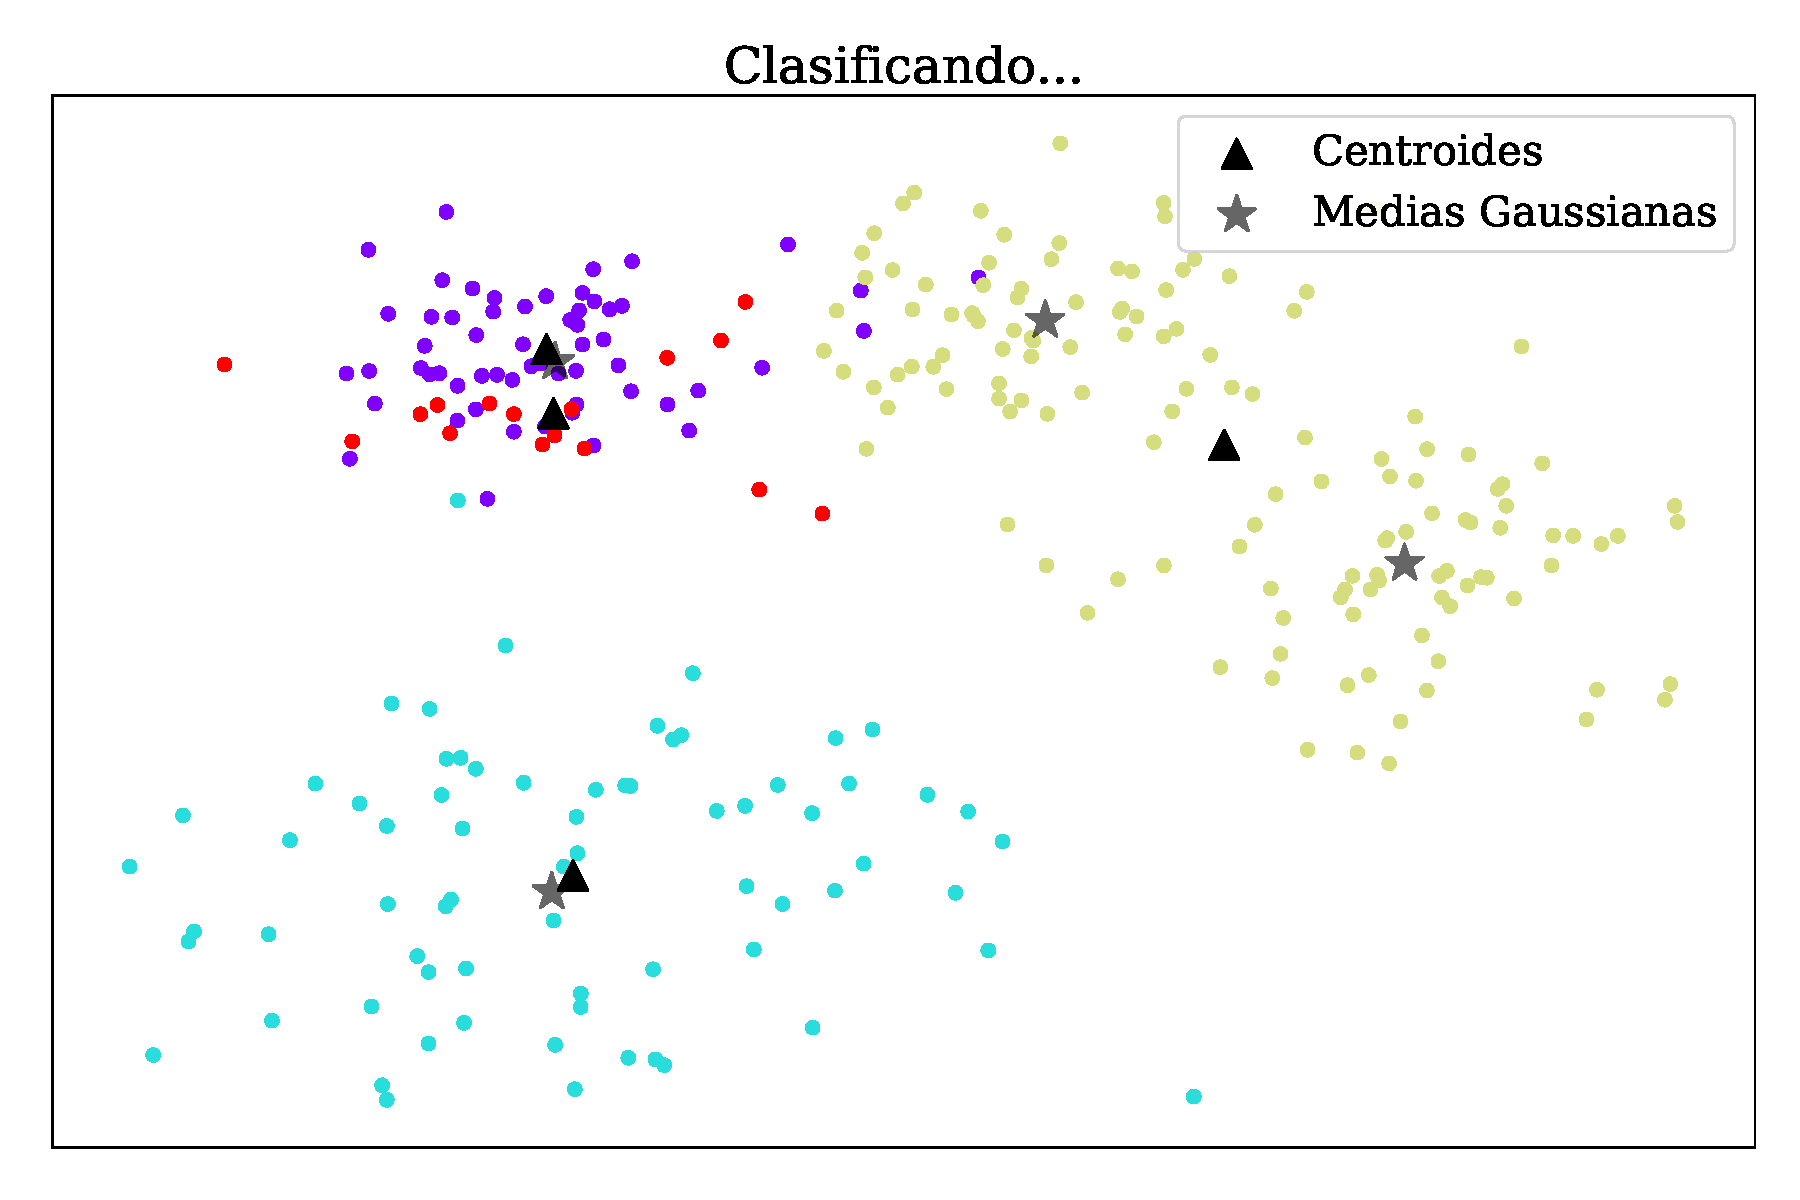
\includegraphics[width=0.5\textwidth]{plots/ejer_2_clasificando_a_conv.pdf}
        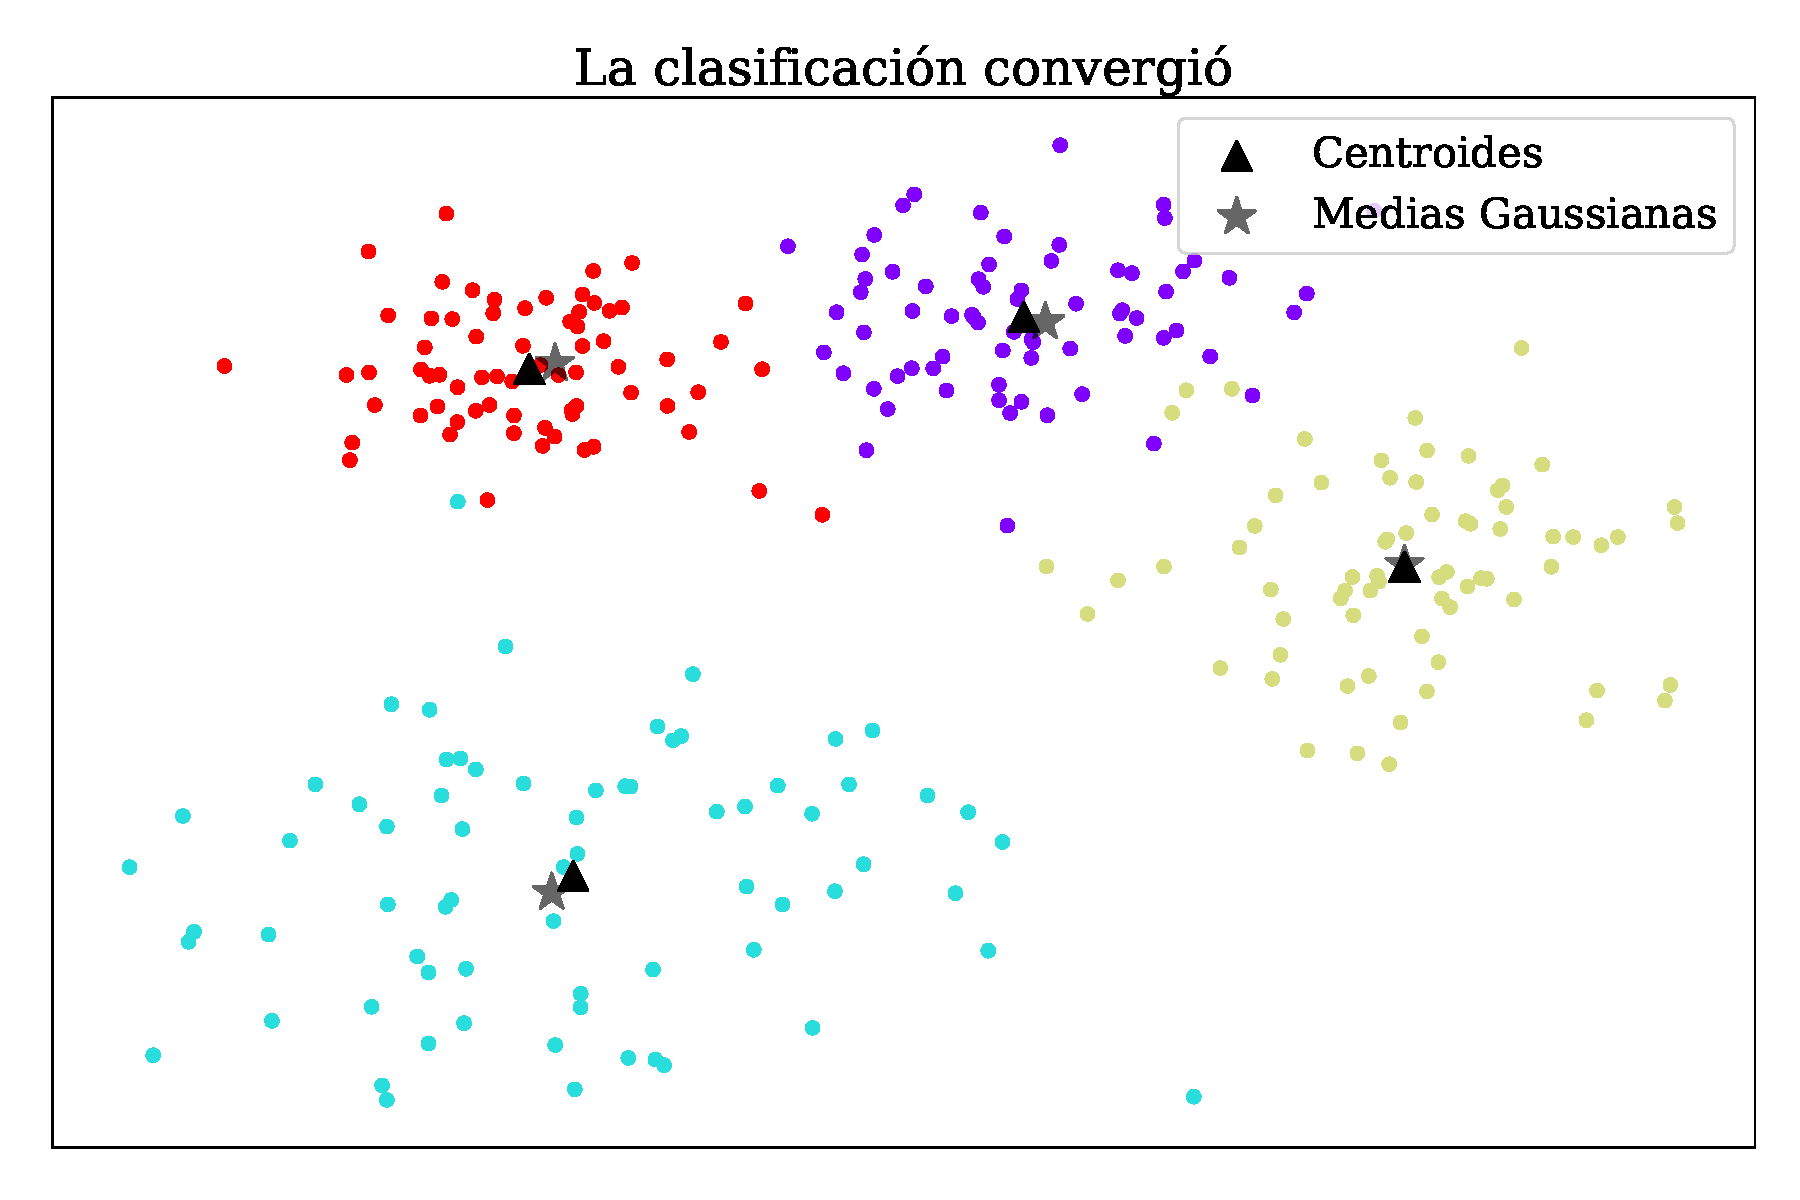
\includegraphics[width=0.5\textwidth]{plots/ejer_2_si_converge.pdf}
        \caption{ejemplos}
        \label{fig:ejer2_converge}
    \end{figure}

    Este es un ejemplo donde no funciona

    \begin{figure}[H]
        \centering
        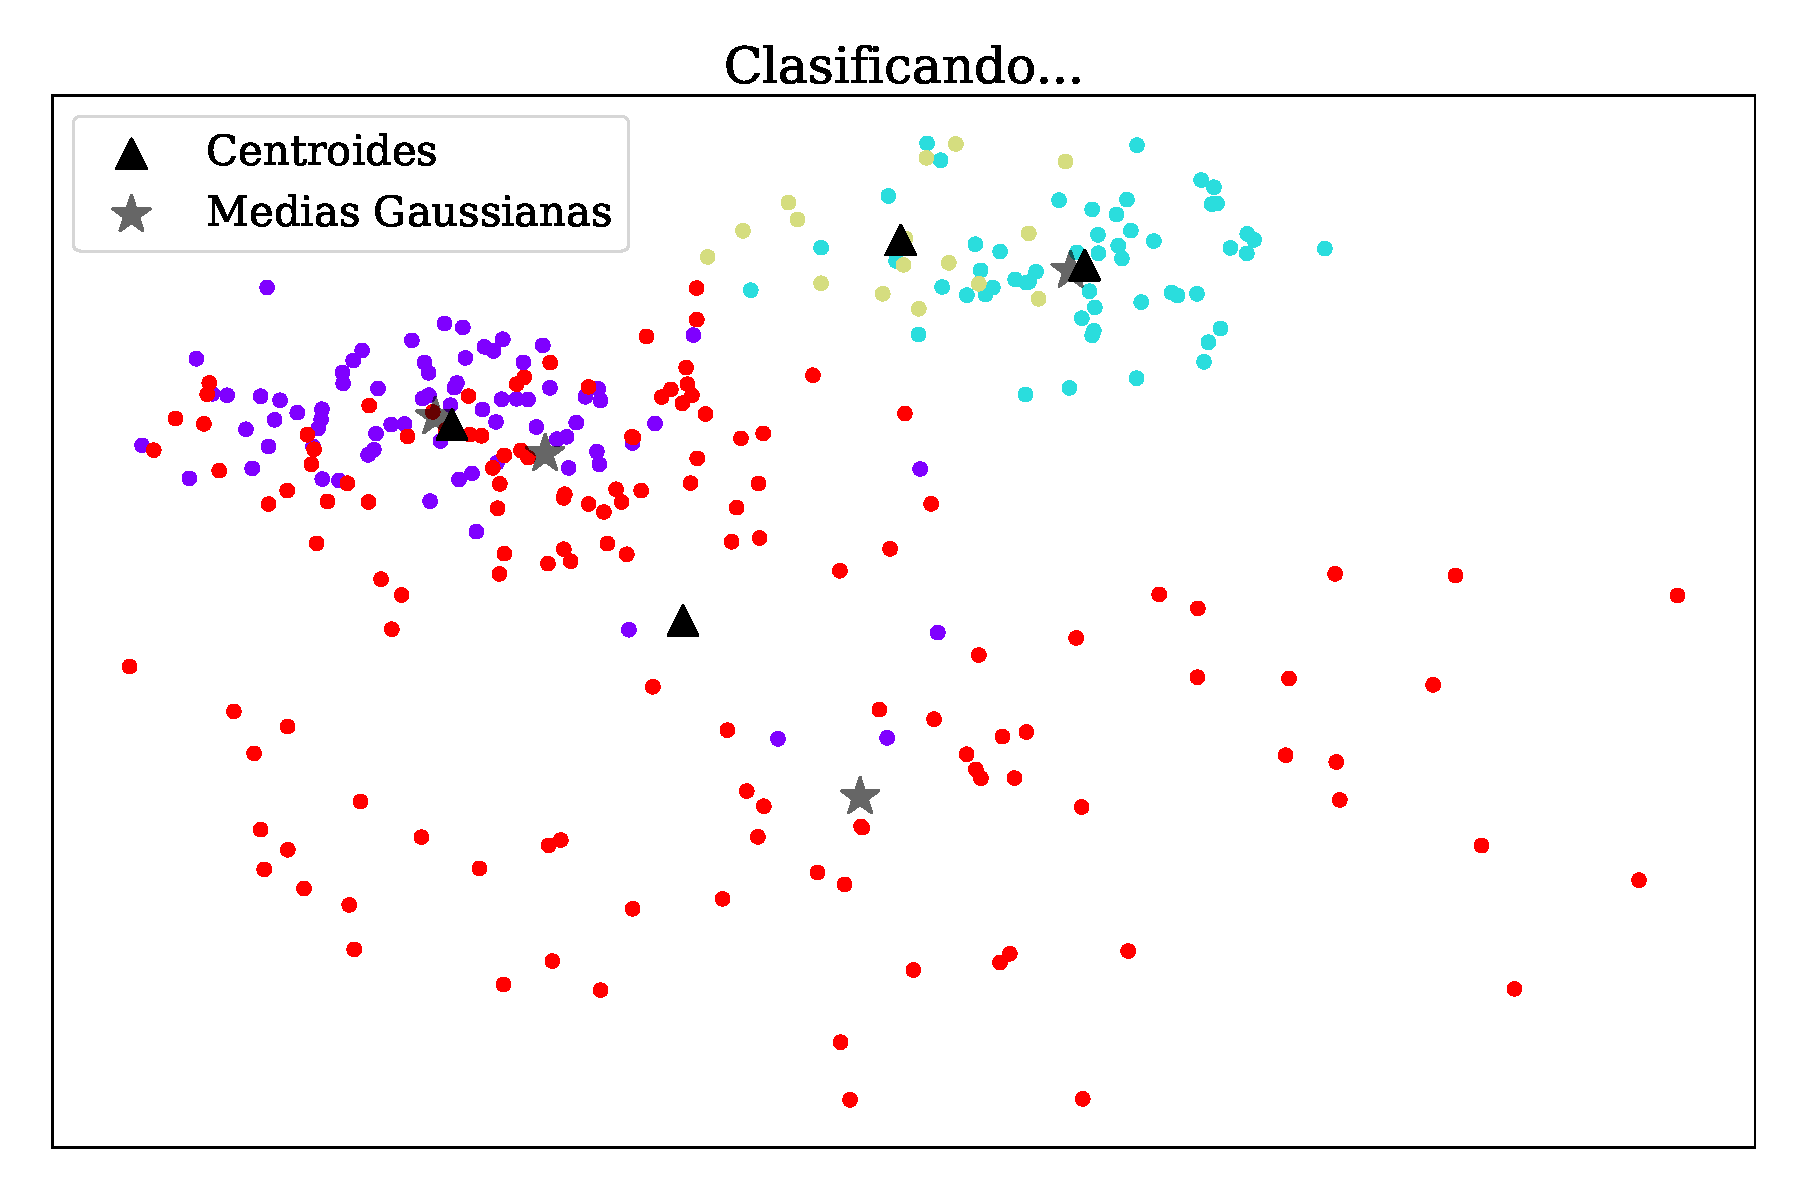
\includegraphics[width=0.5\textwidth]{plots/ejer_2_clasificando.pdf}
        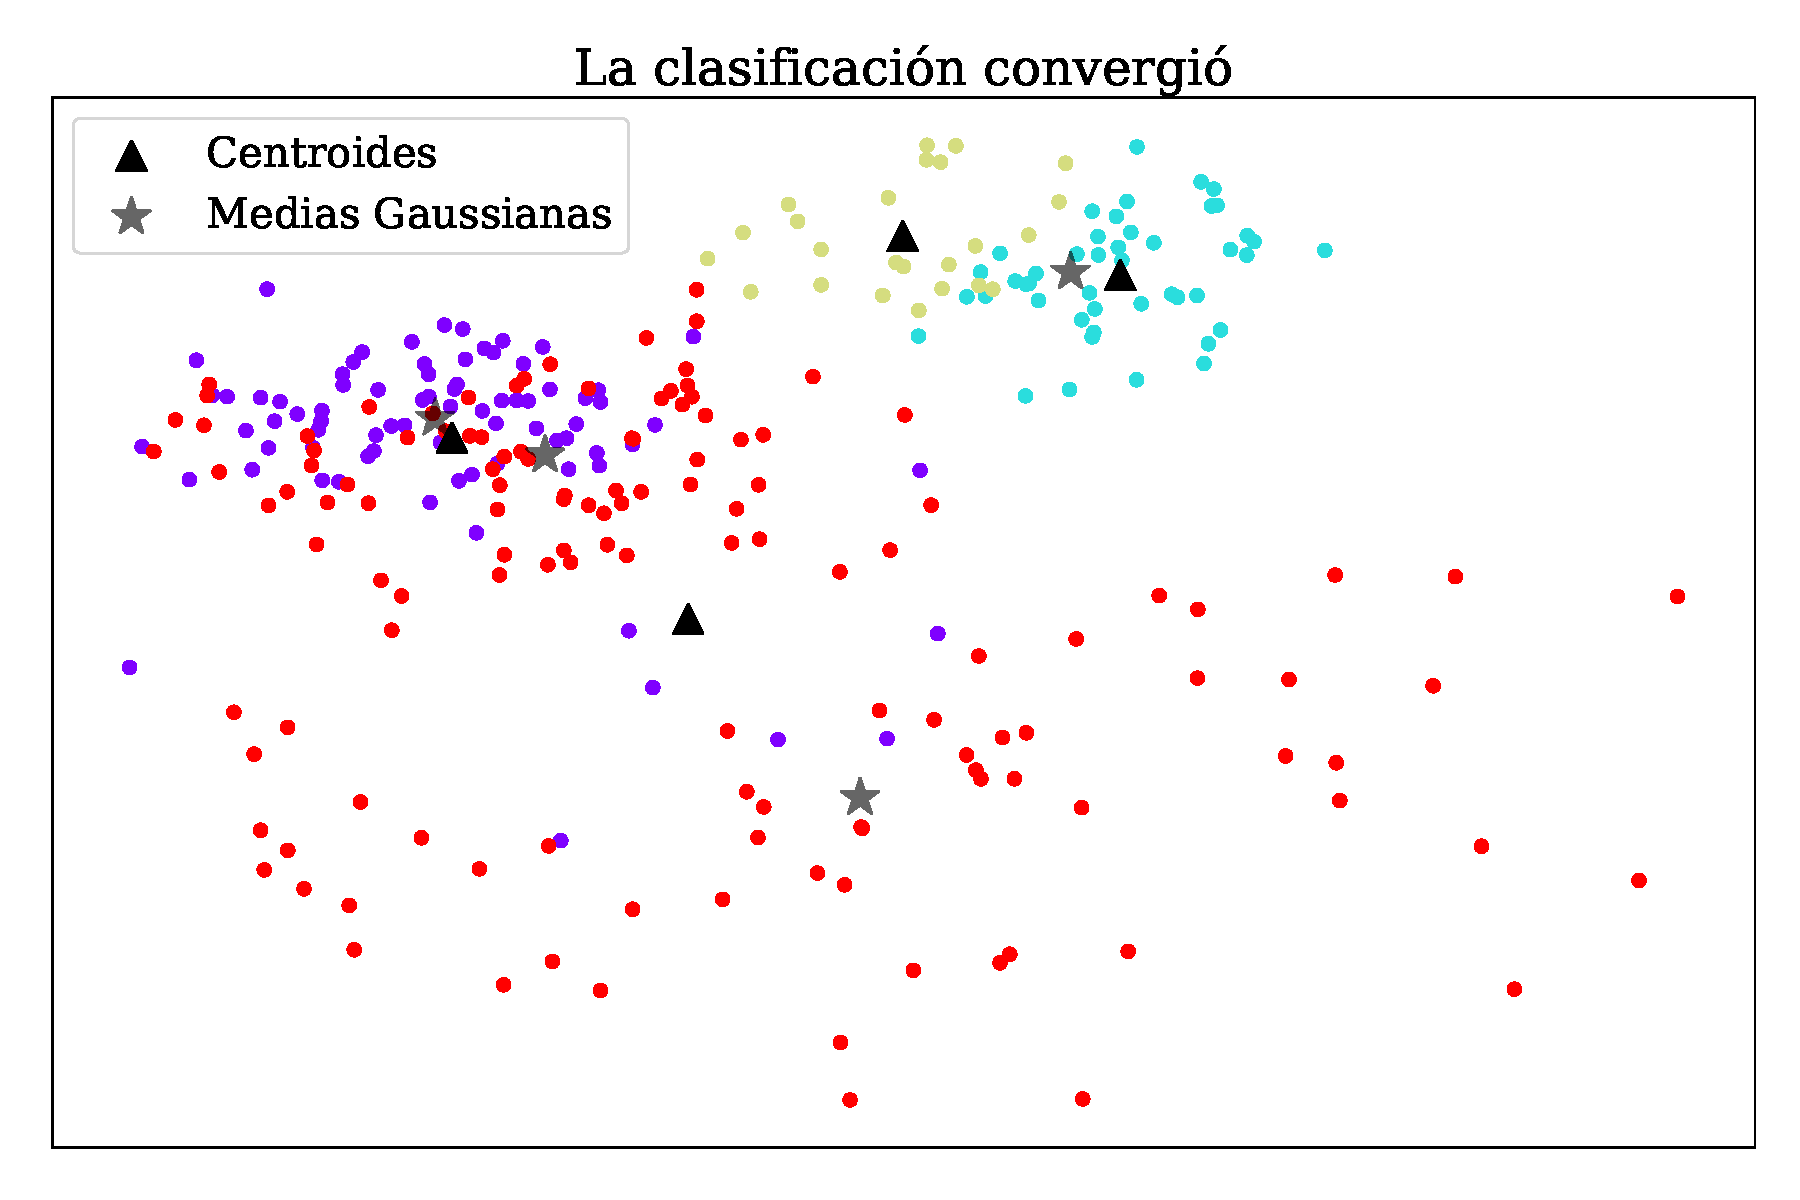
\includegraphics[width=0.5\textwidth]{plots/ejer_2_no_converge.pdf}
        \caption{ejemplos}
        \label{fig:ejer2_no_converge}
    \end{figure}

   \section*{Ejercicio 3}

   Para este ejercicio se utilizó el módulo \emph{datasets} de la librería \emph{Keras} para cargar los datos de entrenamiento y validación del MNIST y CIFAR-10, para utilizar el algoritmo de KNN para la clasificación.

   La ejecución del programa se imprime lo siguiente  en la salida estándar:

   \begin{verbatim}
Con el MNIST: 
Dimensiones del set de entrenamiento:  
(60000, 28, 28)

60000 ejemplos de entrenamiento
10000 ejemplos para probar

100.0% probando con 20 ejemplos


Con el CIFAR-10: 
Dimensiones del set de entrenamiento:
(50000, 32, 32, 3)

50000 ejemplos de entrenamiento
10000 ejemplos para probar

30.0% probando con 20 ejemplos
   \end{verbatim}


    \section*{Ejercicio 4}

    Usando los datos generado para el ejercicio  2 como datos de entrenamiento  y  validación y se implementó el algoritmo KNN para clasificar $375$ puntos,   distribuidos en  5 distribuciones normales  con media y dispersión aleatorias, en dos dimensiones para 1, 3 y 7 vecinos. 

    \subsection*{Número de vecinos k=1}

    Dependiendo de la clasificación de k-means, el algoritmo de KNN puede funcionar o no. En el caso presentado en la Fig.\,\ref{fig:ejer4_k_1_malo} se observa que el k-means separó a los conjuntos de datos coherentemente pero el algoritmo de KNN convergió a  una solución errónea, se presentaron $125$ ejemplos de validación de los cuales el $36\%$ fueron clasificados correctamente.

    \begin{figure}[H]
    \centering
    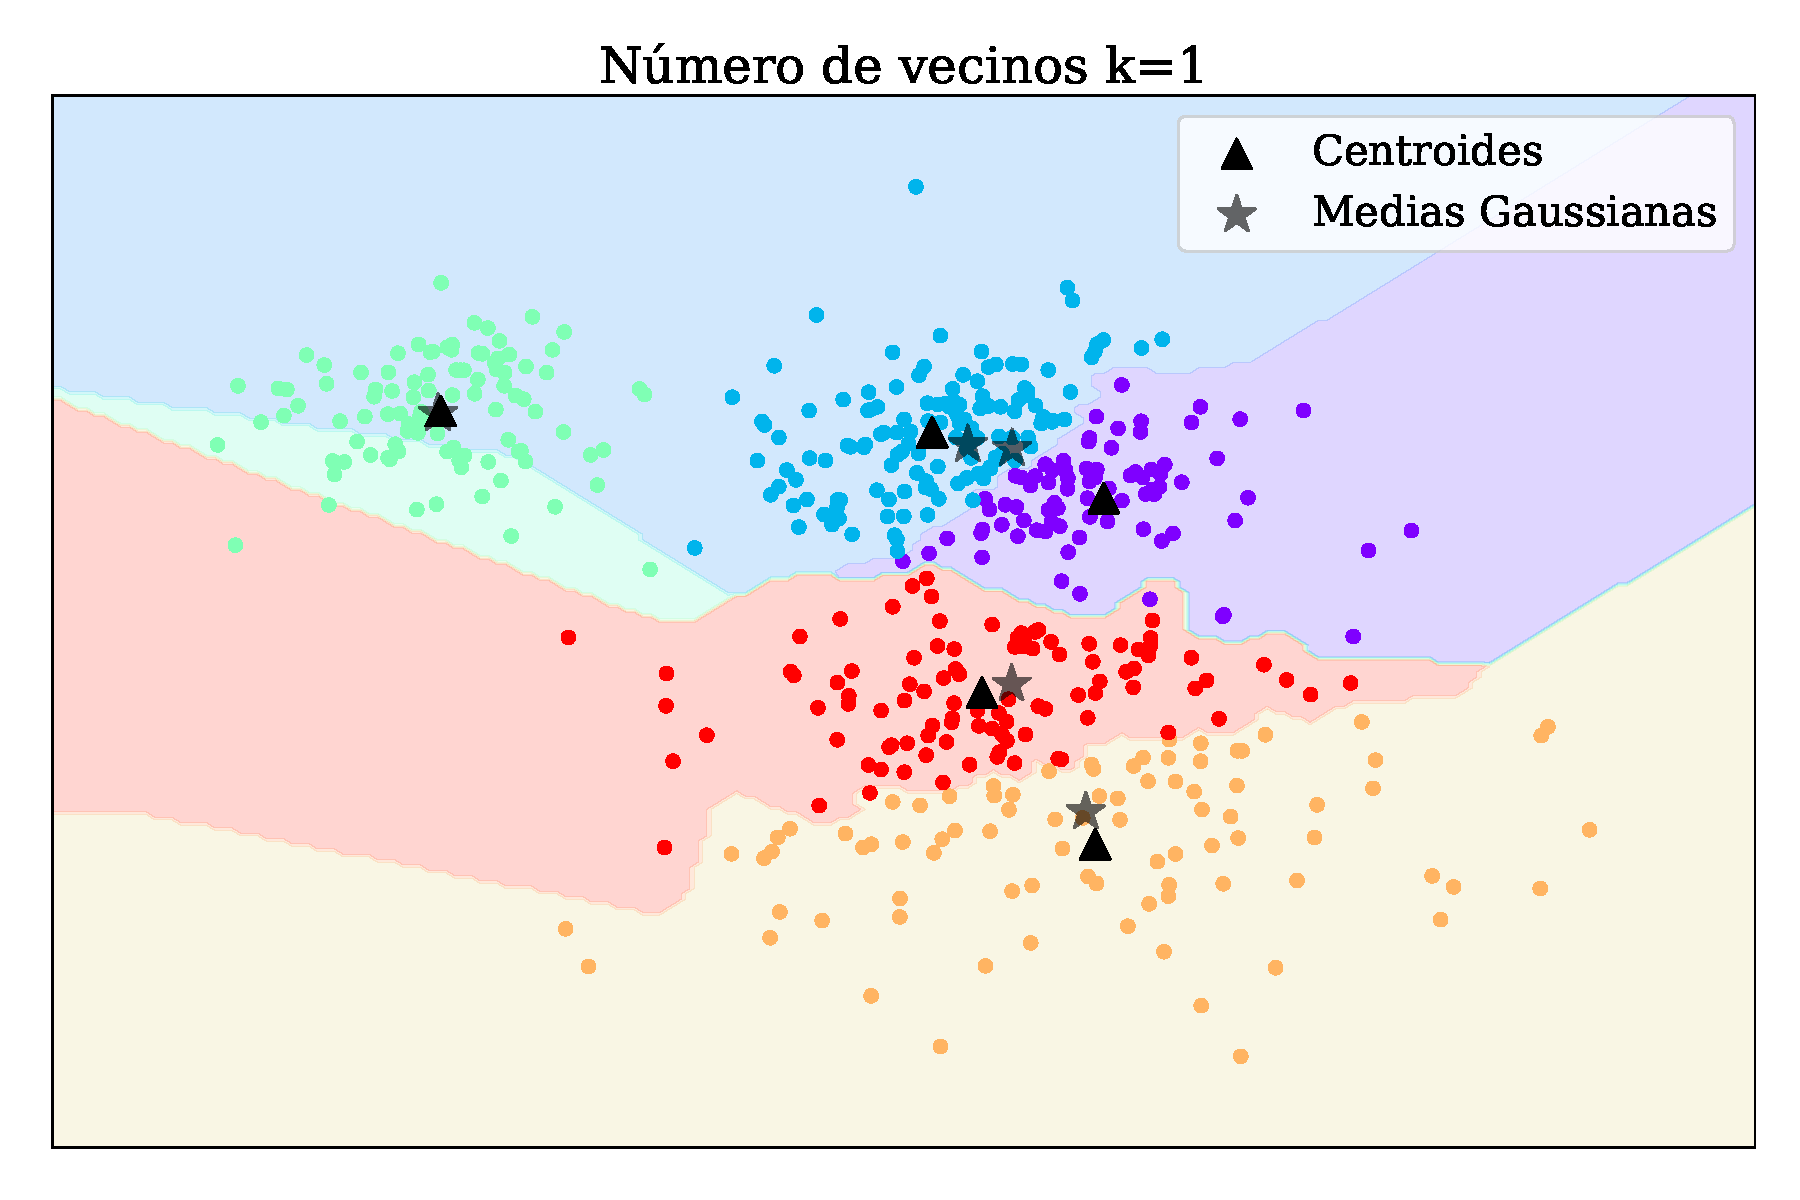
\includegraphics[width=0.5\textwidth]{plots/ejer_4_K-1_no_coverge.pdf}
    \caption{KNN  con K=1, en la validación con 125 datos solo se pudo calificar correctamente el 36.0\%.}
    \label{fig:ejer4_k_1_malo}
    \end{figure} 

    En la Fig.\ref{fig:ejer4_k_1} se observa que el algoritmo converge a una solución, dando $99.2$ de aciertos en los 125 ejemplos de validación.
% k=1
% Dimensiones del set de entrenamiento  (375, 2)
% 375 ejemplos de entrenamiento
% 125 ejemplos para probar

% 99.2\% probando con 125 ejemplos

\begin{figure}[H]
    \centering
    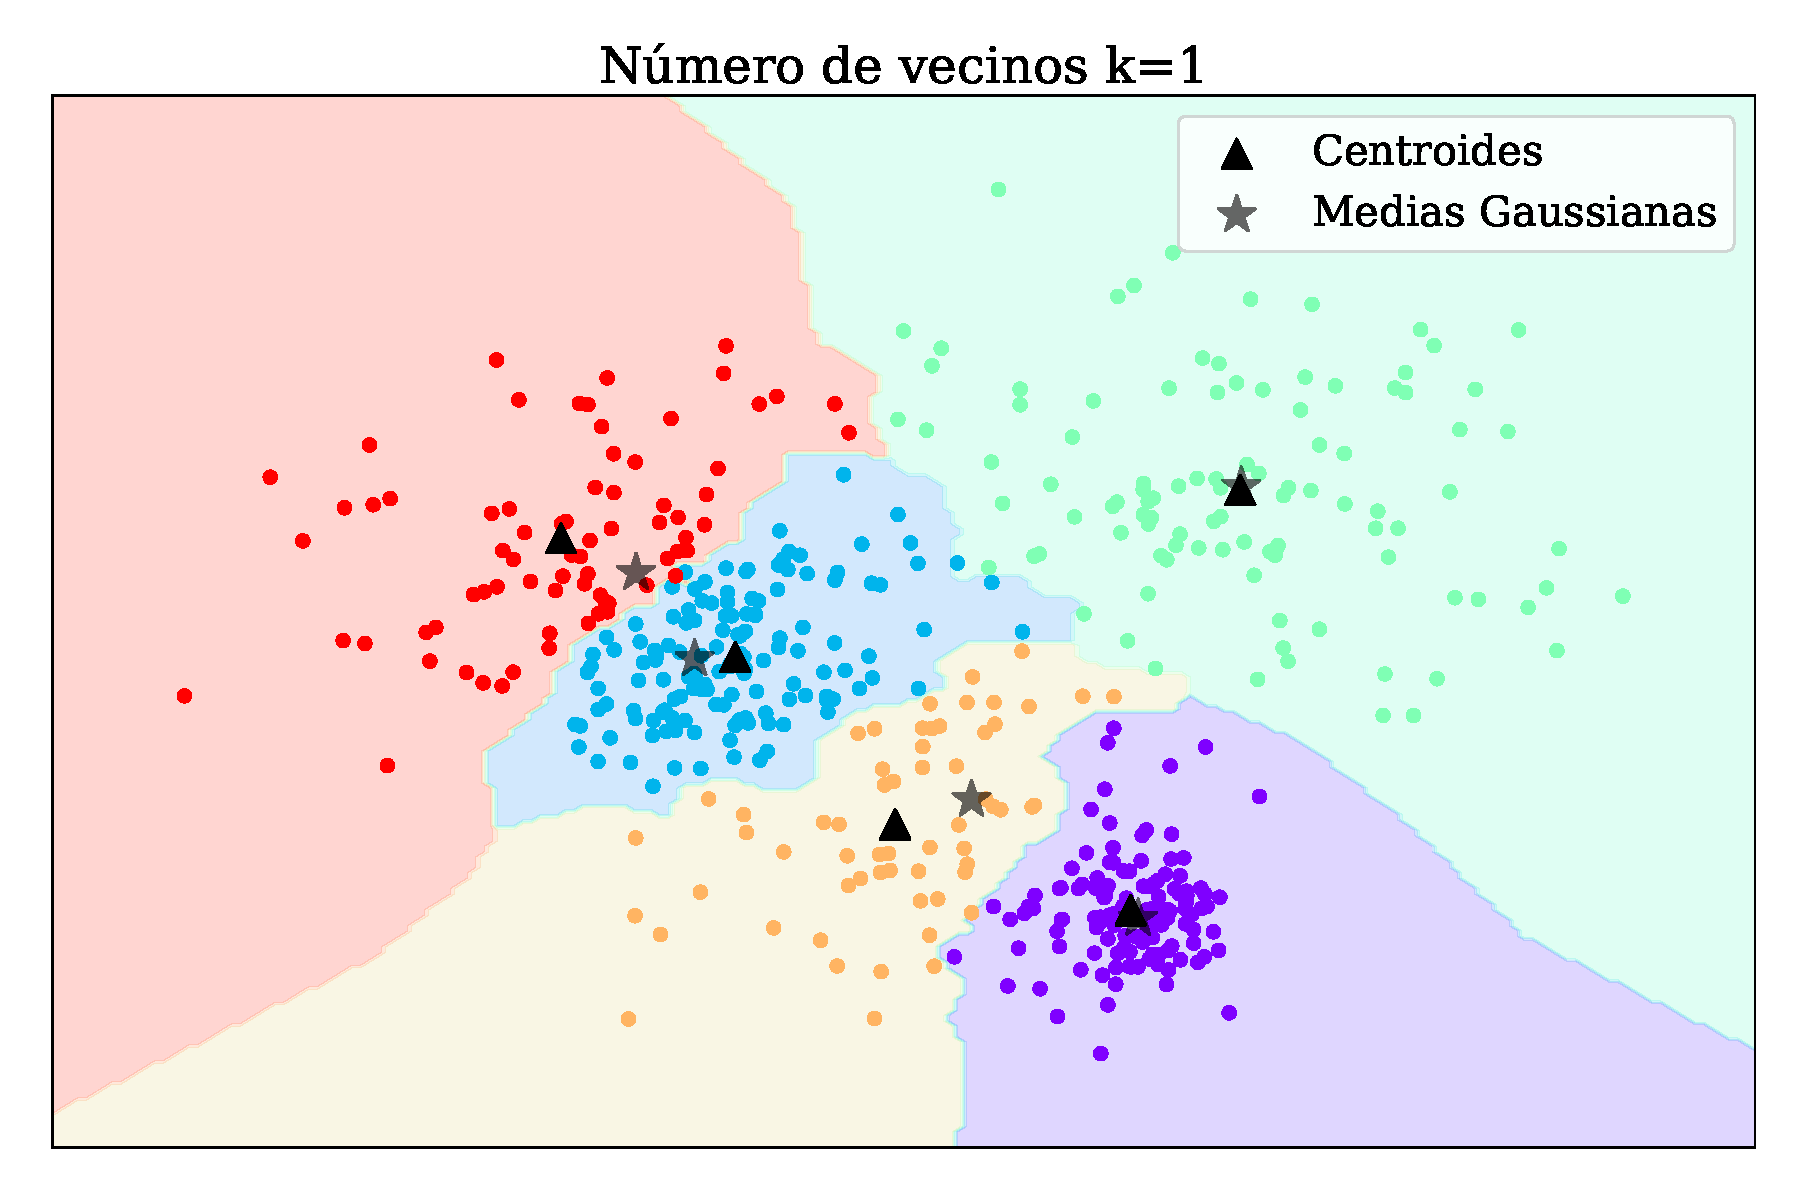
\includegraphics[width=0.5\textwidth]{plots/ejer_4_K-1_si_converge.pdf}
    \caption{K=1 malo}
    \label{fig:ejer4_k_1}
\end{figure} 

    \subsection*{Número de vecinos k=3}

    Para una cantidad de vecinos $k=3$, las  simulaciones y clasificaciones en promedio daban un porcentaje de aciertos menor que k=1. En el caso de la Fig.\,\ref{fig:ejer4_k_3} se obtuvo un 94.4\% probando con 125 ejemplos. 

% k=3
% Dimensiones del set de entrenamiento  (375, 2)
% 375 ejemplos de entrenamiento
% 125 ejemplos para probar



\begin{figure}[H]
    \centering
    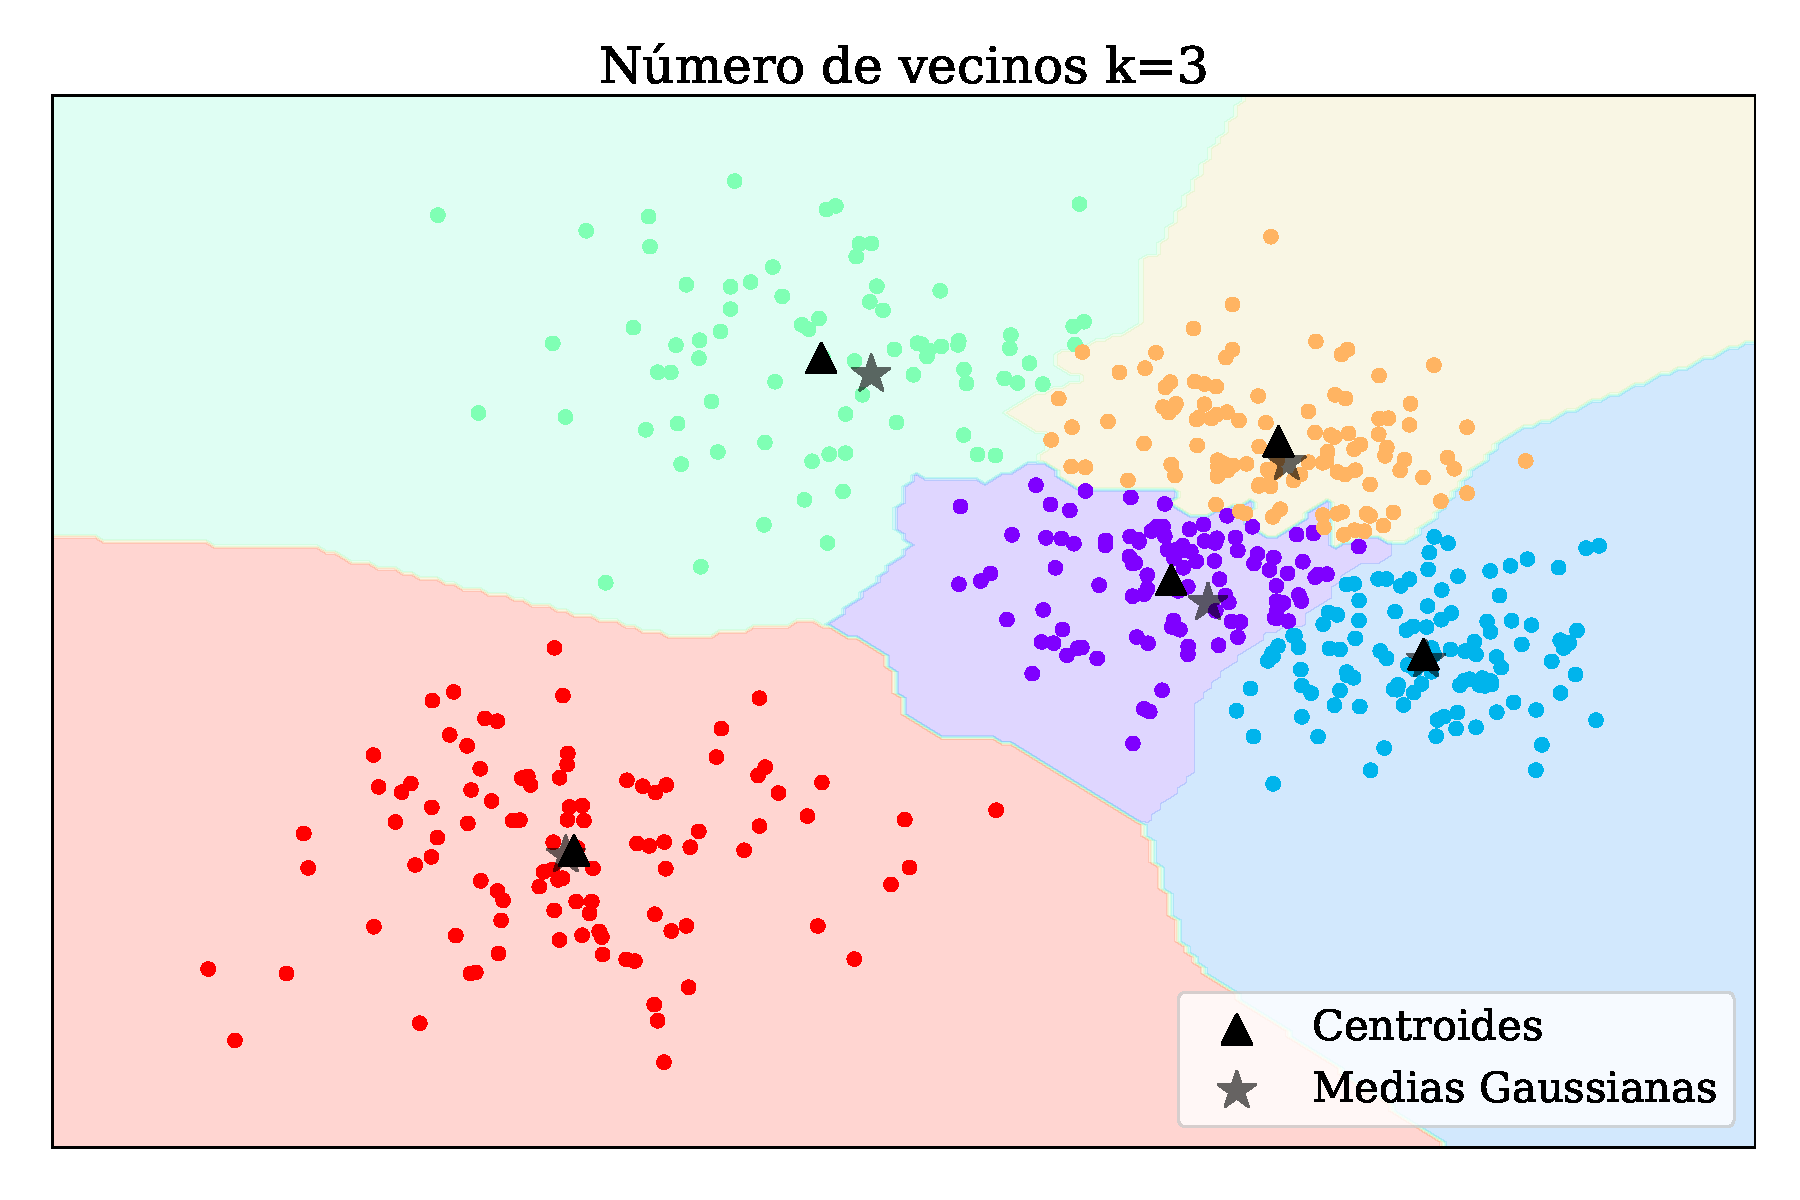
\includegraphics[width=0.5\textwidth]{plots/ejer_4_K-3_si_converge.pdf}
    \caption{K=3 }
    \label{fig:ejer4_k_3}
\end{figure} 

    \subsection*{Número de vecinos k=3}

    Para una cantidad de vecinos $k=7$, el rendimiento de las  simulaciones y clasificaciones en promedio eran peor que los casos anterior. En el caso de la Fig.\,\ref{fig:ejer4_k_7} se obtuvo un 72.0\% probando con 125 ejemplos. Para k=7, la solución a la que converge el algoritmo no tiene la misma generalización que para $k=1$ y $k=3$.


%72.0\% probando con 125 ejemplos
\begin{figure}[H]
    \centering
    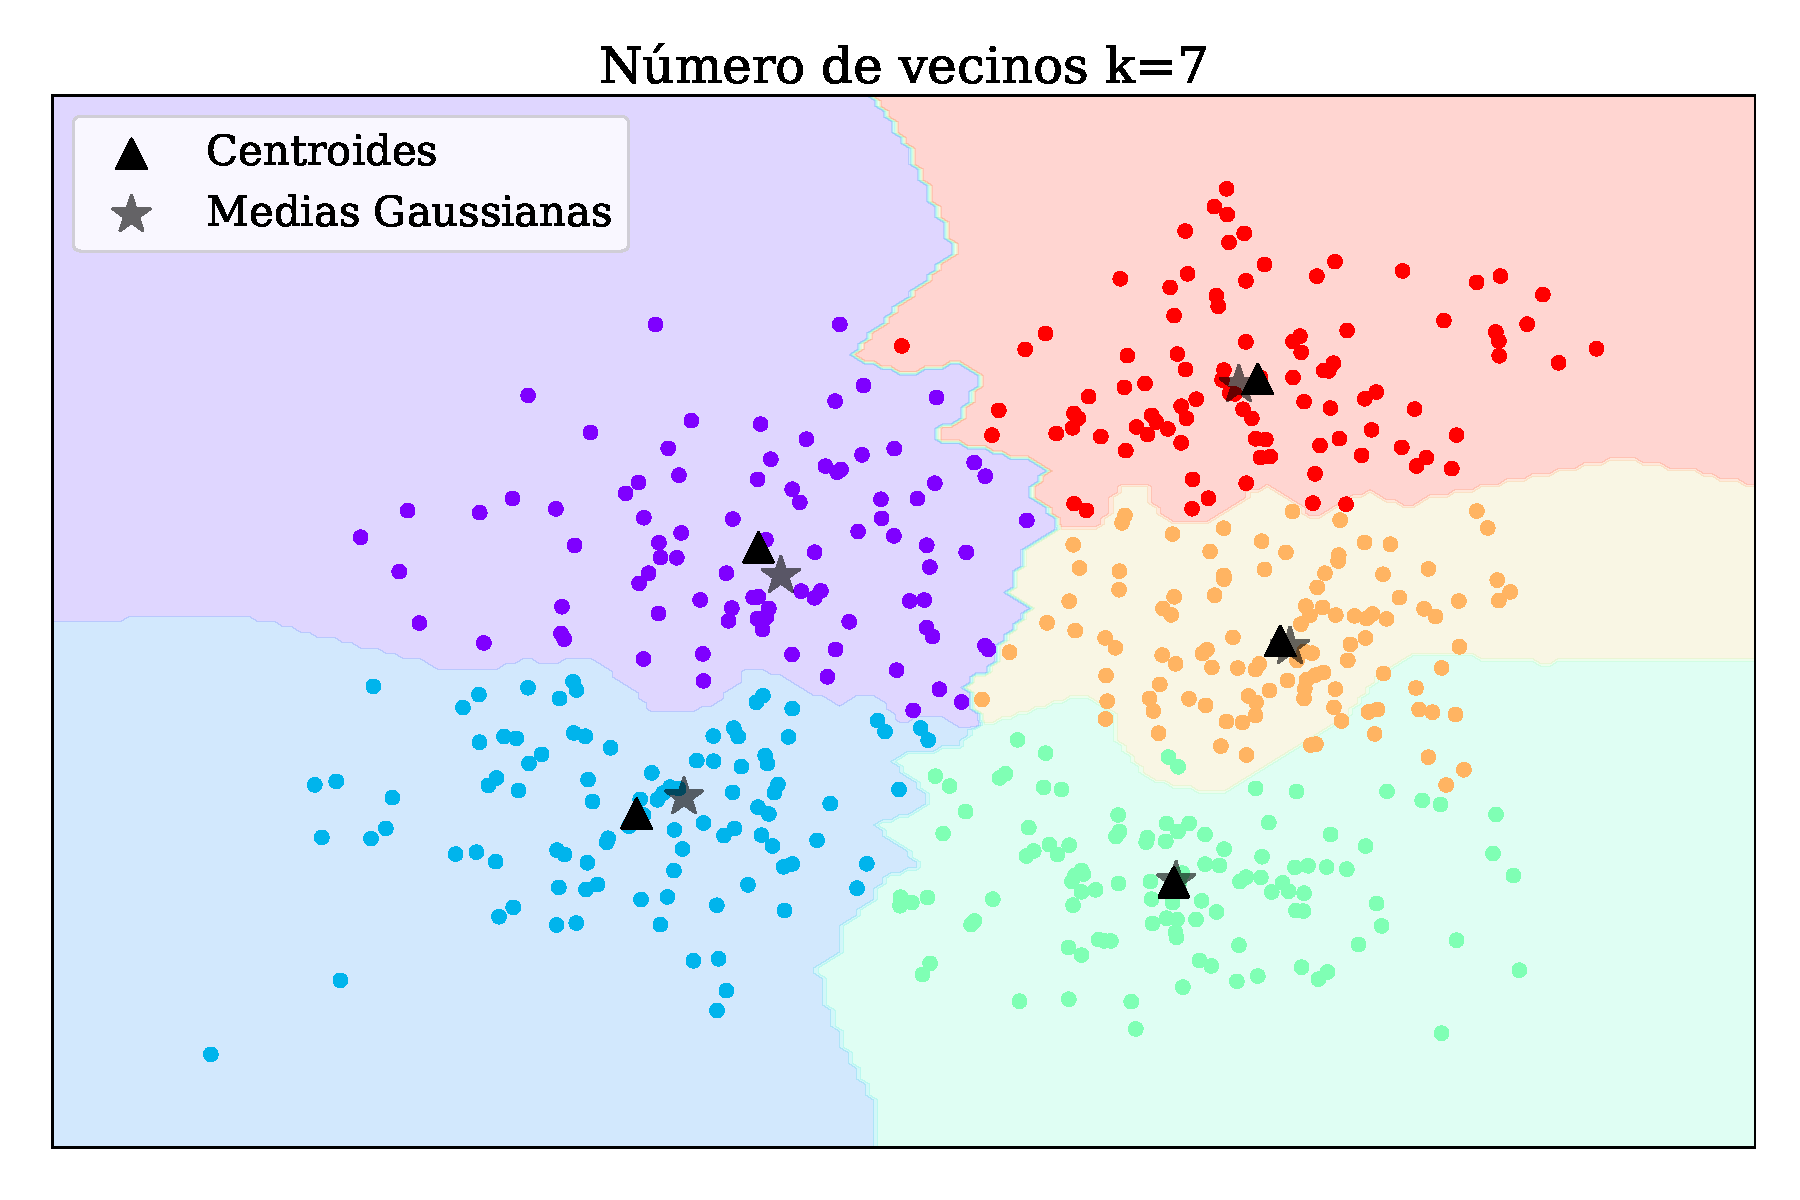
\includegraphics[width=0.5\textwidth]{plots/ejer_4_K-7_si_converge.pdf}
    \caption{K=7 }
    \label{fig:ejer4_k_7}
\end{figure} 
    

\section*{Ejercicio 5}

\begin{figure}[H]
    \centering
    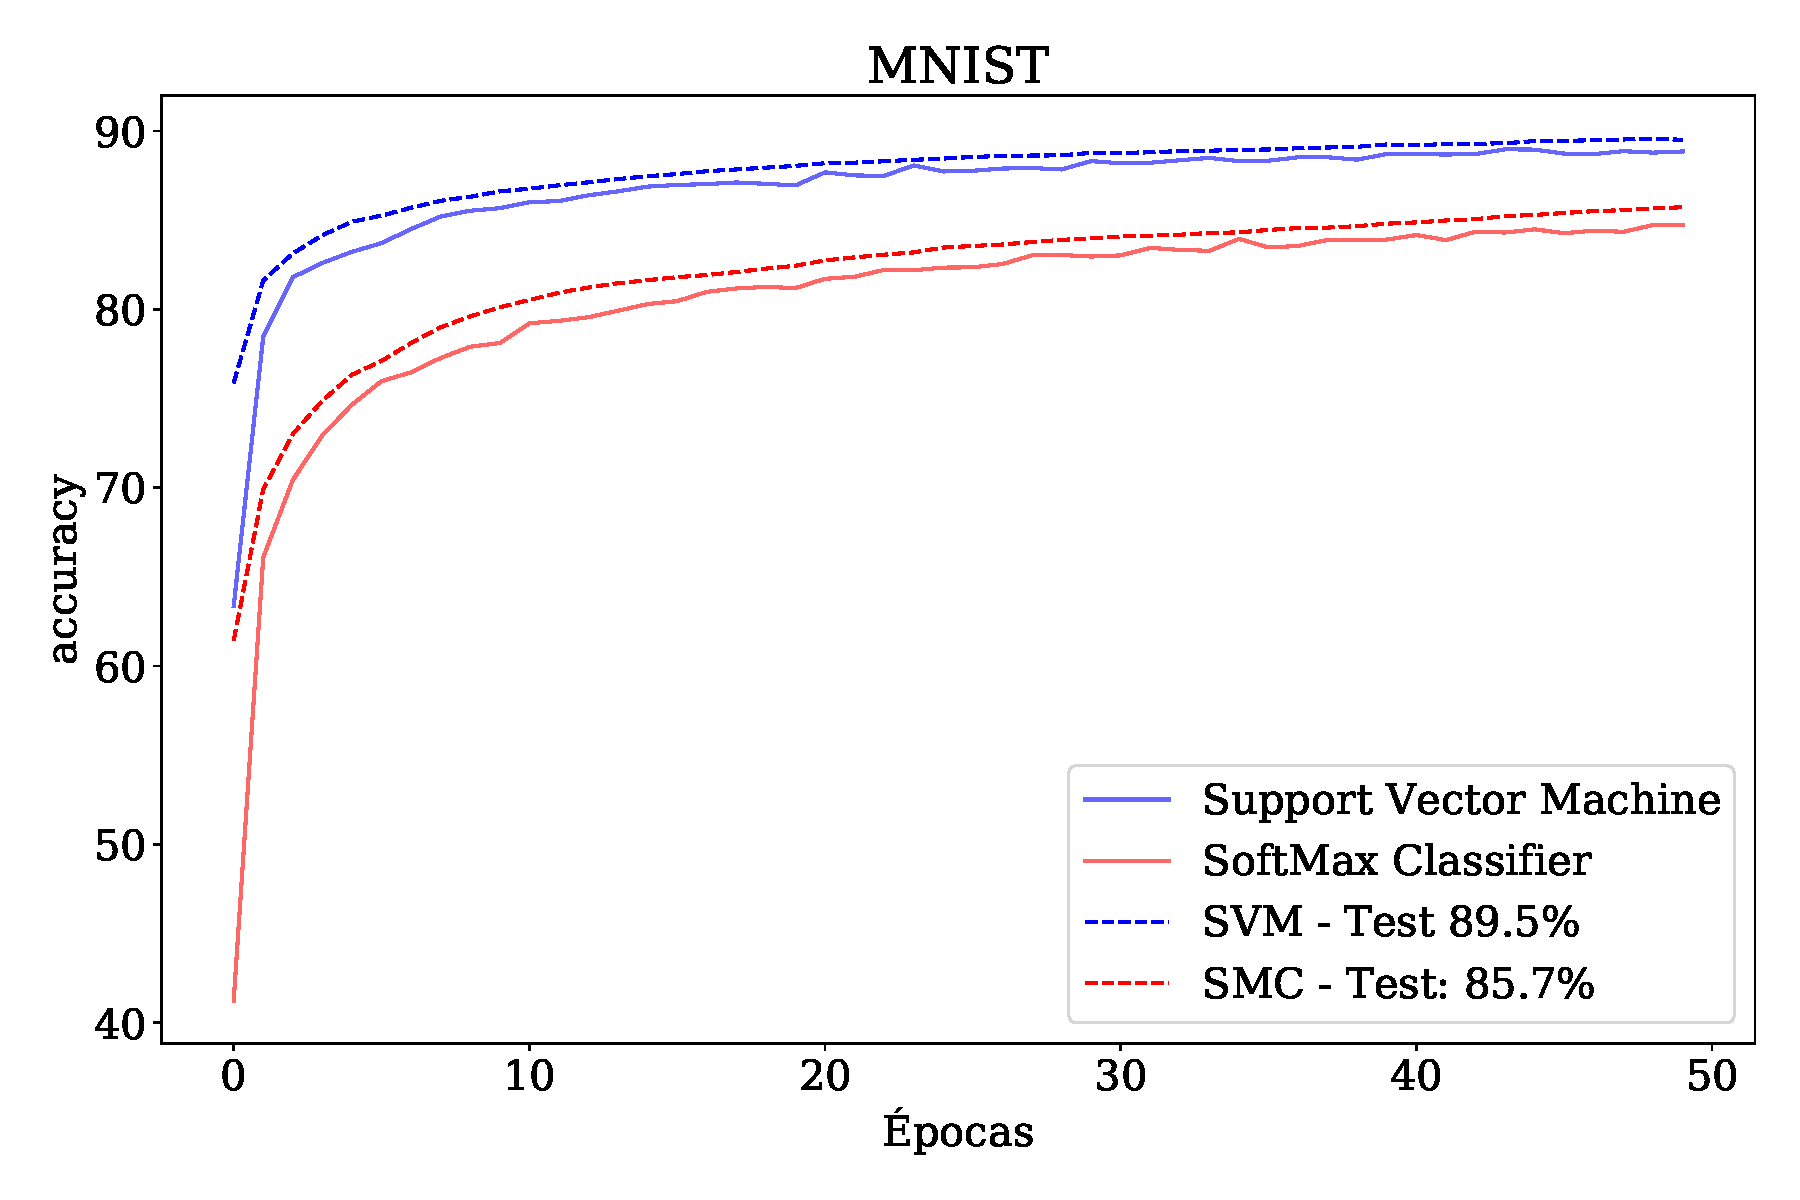
\includegraphics[width=0.5\textwidth]{plots/ejer_5_MNIST_acc.pdf}
    \caption{accuracy}
    \label{fig:ejer5_mnist_acc}
\end{figure} 

\begin{figure}[H]
    \centering
    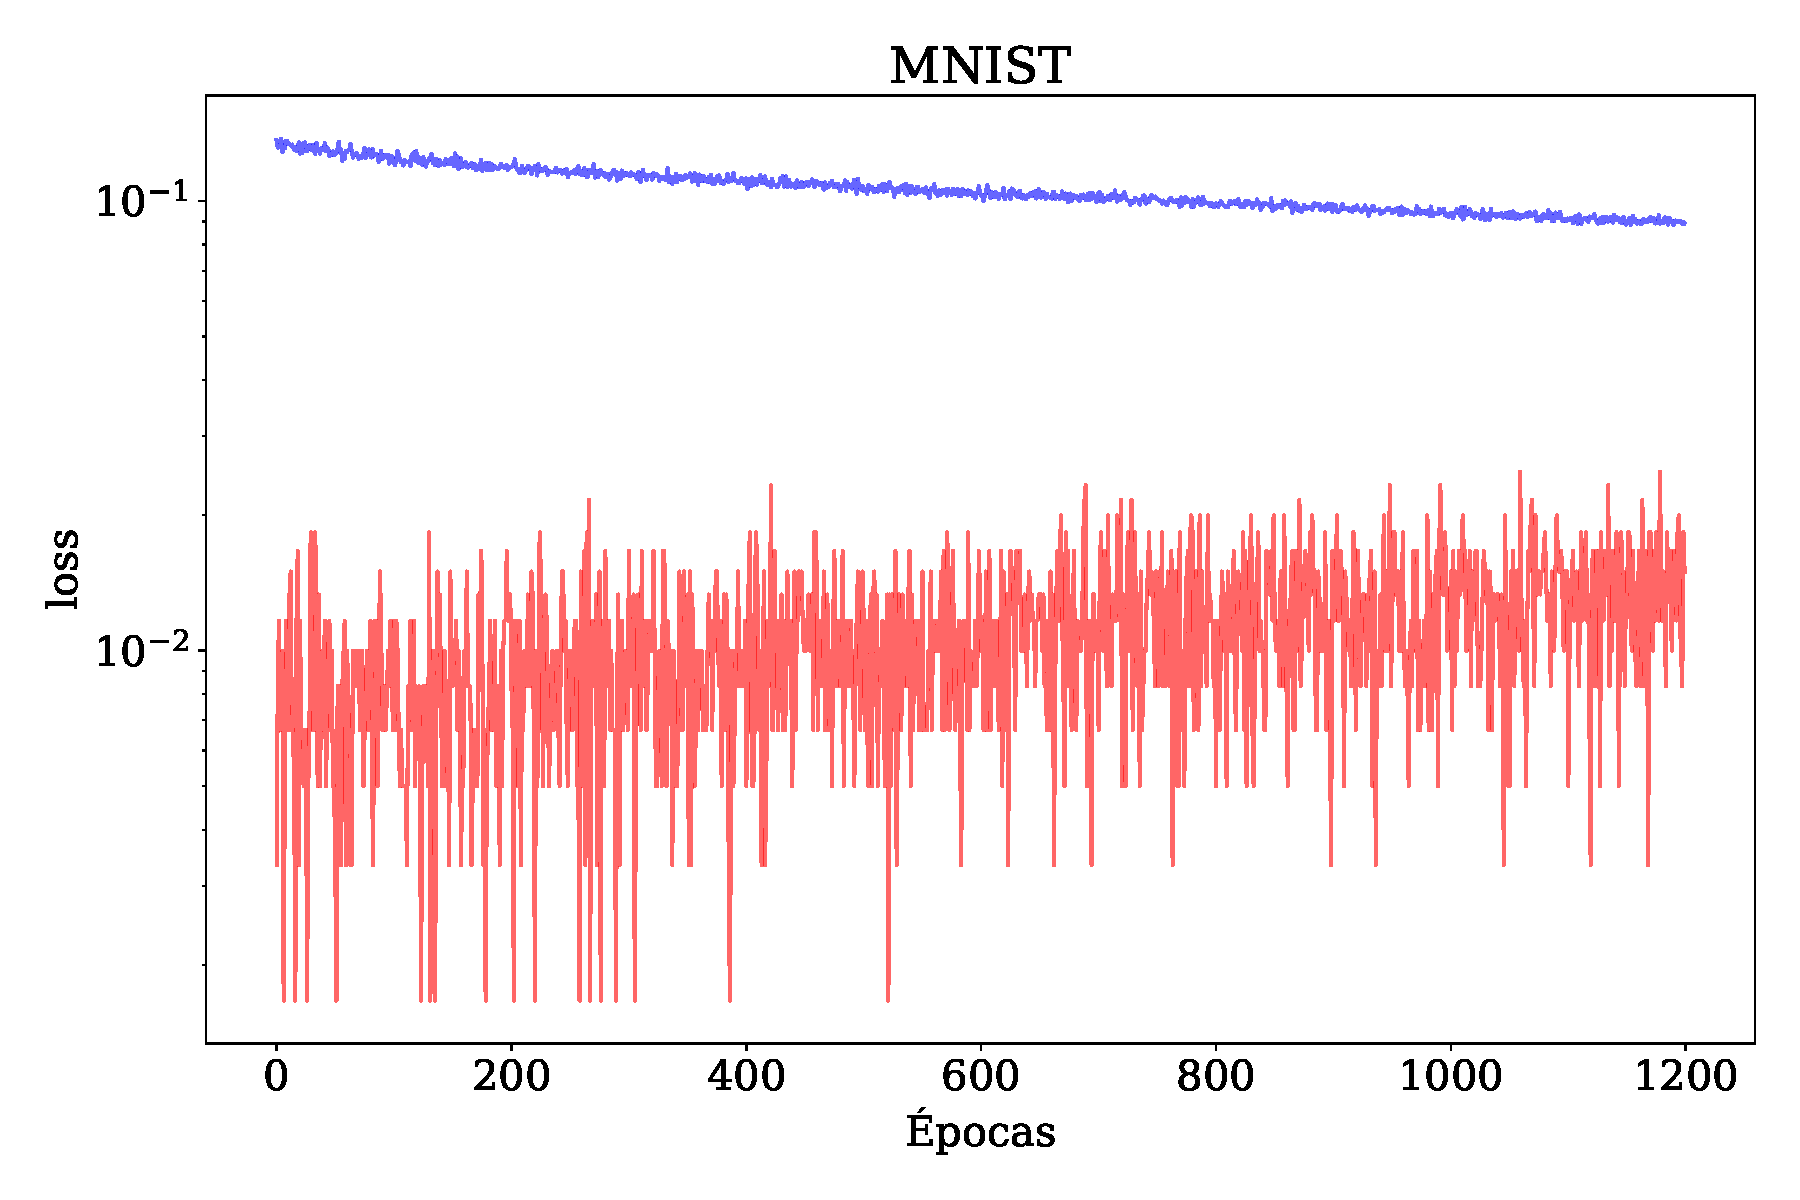
\includegraphics[width=0.5\textwidth]{plots/ejer_5_MNIST_los.pdf}
    \caption{loss}
    \label{fig:ejer5_mnist_loss}
\end{figure} 




\end{document}